\subsection{Mpo manipulations}

The manipulations of MPO's is done by manipulating the tensor into a matrix, performing some matrix calculations and casting it back into it's original form. This section gives some examples how these manipulations are done in practice:

\subsubsection{decomposition}

\def \figone {\expH{2}{$O^{u v,v w}$}{{"$i_1$","$i_2$"}}{{"$j_1$","$j_1$"}}{{"u","w"}}}


\begin{equation}
    \begin{split}
        \figone &= O^{i_1 i_2 j_1 j_2 }_{\alpha_u \gamma_w} \\
        &\cong O^{u w}_{ (\alpha_u i_1 j_1) (\gamma_w i_2 j_2) } \\
        &= O^{u v}_{(\alpha_u i_1 j_1) \beta_v } O^{v w}_{ \beta_v (\gamma_w i_2 j_2) } \\
        &\cong \mpo{2}{{"u","v","w"}}{{"$i_1$","$i_2$"}}{{"$j_1$","$j_1$"}}{}{}
    \end{split}
\end{equation}

Step 2 reshapes and groups the indices to one index. The dimension of this index is the sum of the seperate dimensions. Step 3 decomposes the matrix into a product of 2 matrices. The exact nature of this decomposition is dicussed further. The last step transforms the indices back to separate legs.

For an exact representation, the bond dimension of virtual level v is:
\begin{equation}
    \dim{v} = \min( \dim{u}, \dim{v}) + 2 \dim{i}
\end{equation}


\subsubsection{inverse}
Suppose we want to find a MPO O for given tensors A and B such that the following holds:

\def \figone {\expH{2}{$A$}{{"$i_1$","$i_2$"}}{{"$j_1$","$j_2$"}}{{"u",}}}
\def \figthree {\expH{3}{$B$}{{"$i_1$","$i_2$","$i_3$"}}{{"$j_1$","$j_2$","$j_3$"}}{{"u","v"}}}

\def \figtwo {\mpo{1}{{,"v"}}{{"$i_3$",}}{{"$j_3$",}}{}{}}

\begin{equation}
    \combineTikz{ \figone }{\figtwo}{1.8} =  \figthree
\end{equation}

Again, the indices can be taken toghether in the following way: $\alpha = (u i_1 i_2 j_1 j_2)$ and $\beta = (i_3 j_3 v)$:
\begin{equation}
    A_{\alpha \gamma} O_{\gamma \beta} = B_{\alpha \beta}
\end{equation}

This will be denoted by

\def \figoneb {\expH{2}{$A$}{{,}}{{,}}{{,"w"}}}
\def \figonec {\expH{2}{$A^{-1}$}{{,}}{{,}}{{"w",}}}
\def \figthreeb {\expH{3}{$B$}{{,,"$i_3$"}}{{,,"$j_3$"}}{{,"v"}}}

\def \figtwob {\mpo{1}{{"w","v"}}{{"$i_3$",}}{{"$j_3$",}}{} {}}

\def \figfour { \expH{1}{$A^{-1}B$}{{"$i_3$",}}{{"$j_3$",}}{{"u","v"}} }

\begin{equation}
    \begin{split}
        \figtwob &=  \left[ \figoneb \right ]^{-1}  \figthreeb \\
        &=  \left[ \figonec  \right ]  \figthreeb\\
        &= \figfour
    \end{split}
    \label{eq_mpoinvdef}
\end{equation}

For the first equation the unmarked legs on similar positions need to be connected to each other. The second line the mirrored positions are connected.

This can now be computed with linear algebra packages. Note that it is not necessary to calculate $A^{-1}$ to obtain the solution.
\todo{explain https://nl.mathworks.com/help/matlab/ref/mldivide.html}


\subsubsection{virtual levels and matrisation}

\todo{explain}

\paragraph{Matrisation} From the construction with svd we can see that the dimension of virtual bond $\dim{n} = d^{2 n}$ with d the dimension of $\ket{i}$. The virtual levels can be joined into a $\chi \times d \times d \times \chi$ dimensional tensor O. This tensor is given by a tridiagonal block matrix :

\begin{equation}
    O^{ij}_{\alpha \beta} = \begin{bmatrix}
        O^{00,ij} & O^{01,ij} &           &        &     \\
        O^{10,ij} & O^{11,ij} & O^{12,ij} &              \\
                  & O^{21,ij} & O^{22,ij} & \ddots       \\
                  &           & \ddots    & \ddots &   &
    \end{bmatrix}
\end{equation}

The boundary conditions (leftmost and rightmost virtual level are zero) correspond to vectors:
\begin{equation}
    \begin{split}
        l &= \begin{bmatrix} 1 & 0
              & \cdots\end{bmatrix} \\
        r &= l^{T}
    \end{split}
\end{equation}

The total dimension is the sum of dimensions of the virtual level. In this case the \todo{berken exact en maak tabletje voor de verschillende types}




\subsection{Time evolution methods}

\subsection{Cluster expansion}
This thesis builds on the cluster expansions introduced in \cite{clusterExp}. The idea is to create tensor network with a number of virtual levels. The representation is exact up to M connected sites, where M is the order. Different variations are possible.

A Hamiltonian of the folowing form is assumed
\begin{equation}
    \hat{H}_n = \sum_{i=1}^{n-1} \hat{h} _{i,i+1}+ \sum_{i=1}^n \hat{h'}_i
\end{equation}

Virtual level zero is defined as follows:
\begin{equation}
    \begin{split}
        \mpo{1}{ {0,0}  }{}{}{}{} &=  \expH{1}{}{{,,,,,,,,}}{{,,,,,,,,}}{}
    \end{split}
\end{equation}




Similarly, the contraction of elements $O_{01}$ and $O_{10}$ are defined as follows:

\begin{equation}
    \mpo{2}{{0,1,0}}{}{}{}{} =  \expH{2}{}{}{}{} - \mpo{2}{{0,,0}}{}{}{}{}
\end{equation}

Some notation will be introduced that will be used later on. The rensor $L_n$ is the contraction of n MPO's where the virtual index increases between each bond. $R_n$ is similar but the virtual bond starts from n and decreases.

\def \On {\mpo{4}{ {0,1,,"m","n"}  }{}{}{{0,0,1,0,0}}{}}
\def \OnBlock {\expH{4}{ $L_n$  }{ {,,"...",} }{ {,,"...",} }{{0,"n"}} }

\begin{equation}
    \begin{split}
        &\OnBlock = \On\\
    \end{split}
\end{equation}



\def \MnBlock {\expH{4}{ $M_n$  }{ {,,"...",} }{ {,,"...",} }{}{} }
\def \expHBlock {\expH{4}{ $e^{- \beta \hat{H}_{n}}$   }{ {,,"...",} }{ {,,"...",} }{}{} }
\def \Mn {\mpo{4}{ {0,,,,0}  }{}{}{{0,0,1,0,0}}{}}

$M_n$ is the difference between the exponentiated hamiltonian for n sites and the contraction of the MPO over all the currently assigned combinations of virtual levels.

\begin{equation}
    \begin{split}
        \MnBlock &=  \expHBlock \\
        &-\Mn \\
    \end{split}
\end{equation}

\subsubsection{Type A}
This type was originally proposed in \cite{clusterExp}. The following types of blocks appear:

\mpo{1}{ {"n","m"}  }{}{}{}{},\mpo{1}{ {"m ","n"}  }{}{}{}{} and \mpo{1}{ {"n","n"}  }{}{}{}{} with $n \in \mathbb{N}_0$ and $m=n-1$.

\paragraph{$O^{n n}$}

The $O^{n n}$ block is defined by \cref{eq_nn_level}


\def \rhs{\expH{1}{ $L_{n}^{-1}  M_{2n+1}  R_{n}^{-1}$ }{}{}{{"n","n"}}  }

\begin{equation}
    \mpo{1}{ {"n","n"}  }{}{}{}{} = \rhs
    \label{eq_nn_level}
\end{equation}

The residual error M is calculated for a chain of size $2n+1$. The left and right inverses are applied to M to find the block $O^{n n}$

\paragraph{ $O^{m n }$ and $O^{n m} $}
The contraction of $O^{n m }$ and $O^{m n} $ is defined by:


\def \rhs{\expH{1}{ $L_{n}^{-1}  M_{2n+2}  R_{n}^{-1}$ }{}{}{{"n","n"}}  }
\begin{equation}
    \mpo{2}{ {"n","m","n"}  }{}{}{}{} = \rhs
    \label{eq_nmn_level}
\end{equation}

The individual elements $O^{m n }$ and $O^{n m} $ are obtained by doing an svd decoposition.

\todo{symmetric split S, invertibility lowest eiges, eigensplit, order cutoff}

During the svd the bond dimension can be lowered by only keeping the rows and colums belonging to $\sigma > \sigma_0$. This also helps the invertibility. Increasing $\sigma_0$ reduces the precision of the MPO. This can be seen in \cref{fig:sigman0}. A good tradeoff seems to be $ \sigma_0 = {10}^{-12}$. There is almost no precision loss vor small $\beta$, while for intermediate it performs optimal for intermediate $\beta$.


\begin{figure}
    \centering
    \begin{subfigure}{\textwidth}
        \centering
        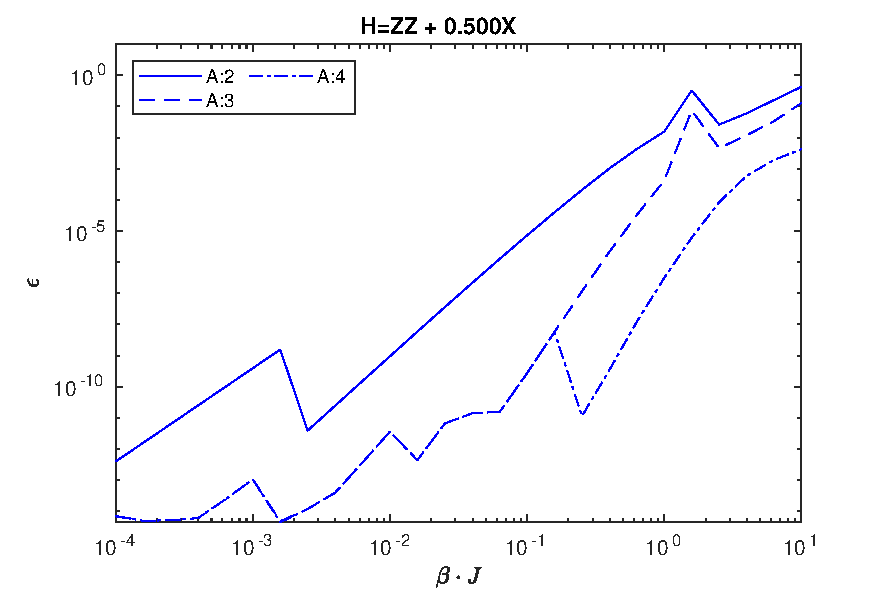
\includegraphics[width=0.8\linewidth]{Figuren/mpo_construction/sigm0/e10.pdf}
        \caption{ ${10}^{-10}$}
        \label{fig:sub1}
    \end{subfigure}%

    \begin{subfigure}{\textwidth}
        \centering
        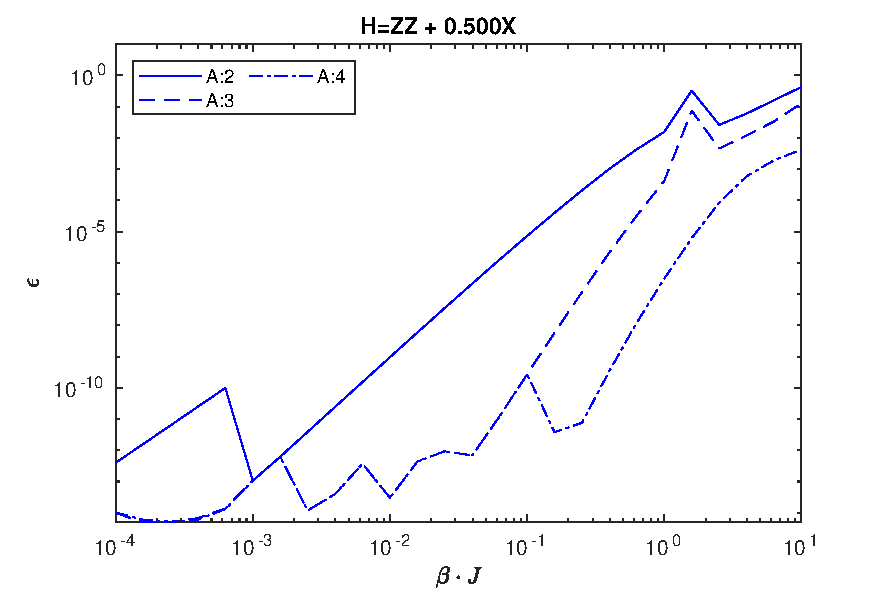
\includegraphics[width=0.8\linewidth]{Figuren/mpo_construction/sigm0/e11.pdf}
        \caption{${10}^{-11}$}
        \label{fig:sub2}
    \end{subfigure}
    \caption{A figure with two subfigures}
    \label{fig:sigman0}
\end{figure}


\begin{figure} \ContinuedFloat
    \centering
    \begin{subfigure}{\textwidth}
        \centering
        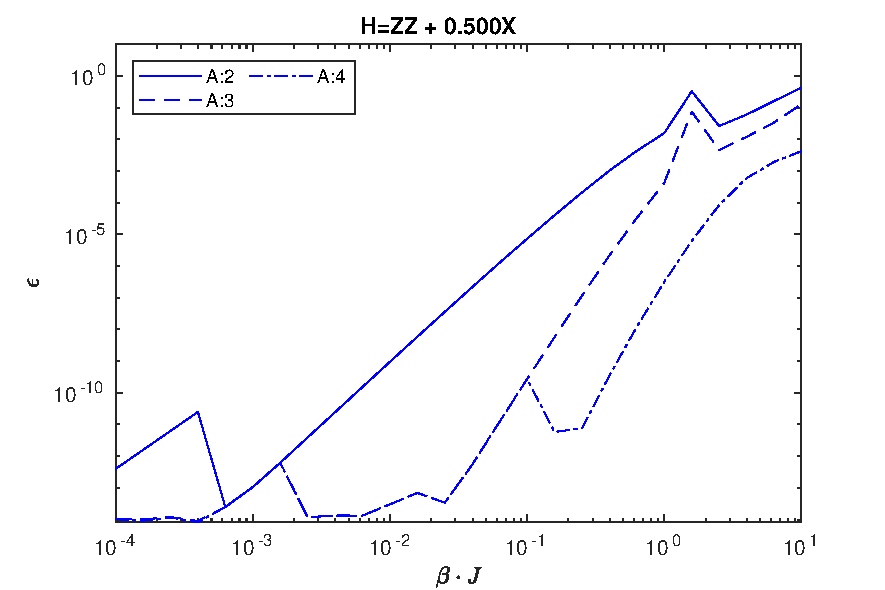
\includegraphics[width=0.8\linewidth]{Figuren/mpo_construction/sigm0/e12.pdf}
        \caption{ ${10}^{-12}$}
        \label{fig:sub1}
    \end{subfigure}%

    \begin{subfigure}{\textwidth}
        \centering
        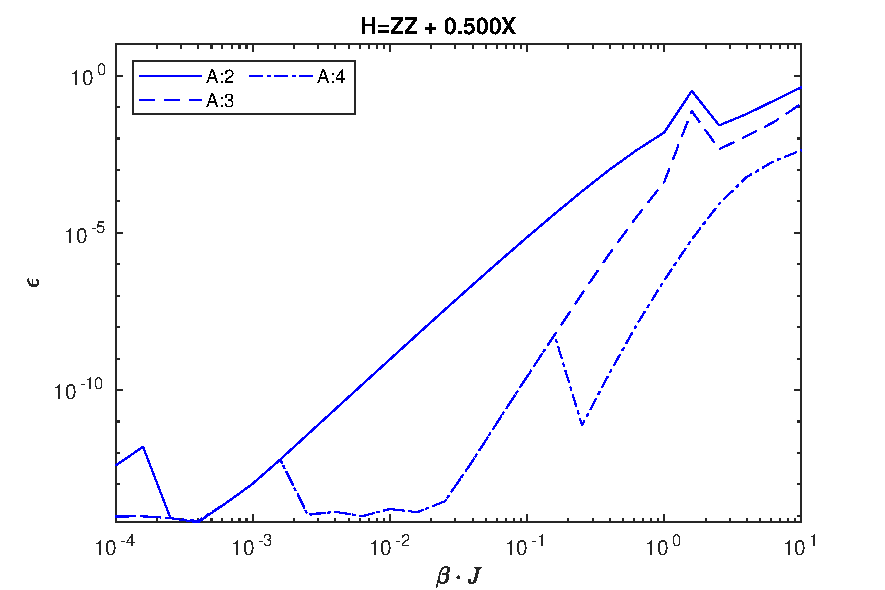
\includegraphics[width=0.8\linewidth]{Figuren/mpo_construction/sigm0/e13.pdf}
        \caption{${10}^{-13}$}
        \label{fig:sub2}
    \end{subfigure}
    \caption{A figure with two subfigures}
    \label{fig:sigman0}
\end{figure}


\begin{figure} \ContinuedFloat
    \centering
    \begin{subfigure}{\textwidth}
        \centering
        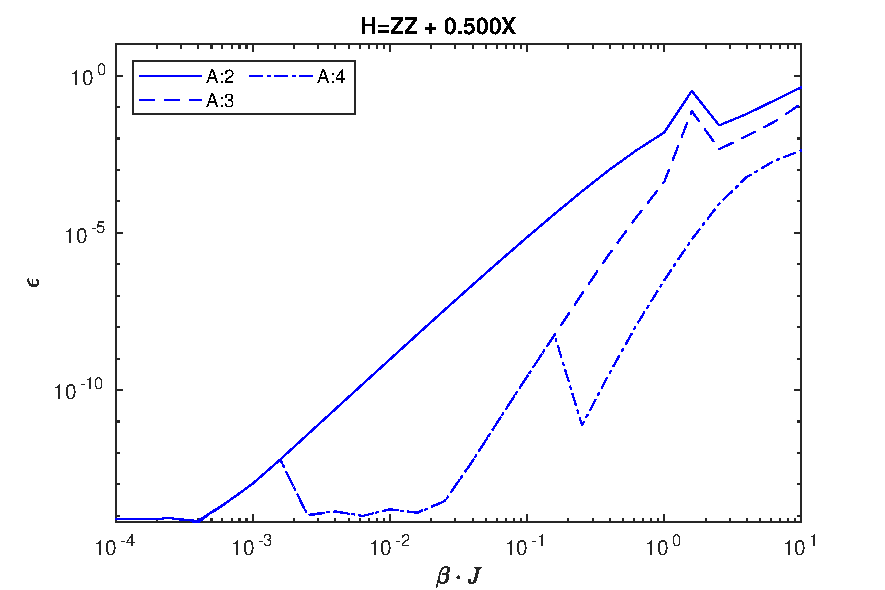
\includegraphics[width=0.8\linewidth]{Figuren/mpo_construction/sigm0/e14.pdf}
        \caption{ ${10}^{-14}$}
        \label{fig:sub1}
    \end{subfigure}%
    \caption{A figure with two subfigures}
    \label{fig:sigman0}
\end{figure}

\todo{toon figuurtjes met verschillende sigma 0 voor $t_ising$}



As can be seen in \cref{construction:sigma0}, mainly the construction for small values of $\beta$ get affected by the choice of $\sigma_0$.


\subsubsection{Truncation}

\paragraph{ \( O^{n n} \)}


Intoduction of a \( O^{n n} \) block can result in large fluctuating errors. This happens because the inverses are possible ill conditioned. Therefore the construction of the MPO should be stopped at a certain optimal order.


% For this block 2 criteria need to be checked. First, the inverse needs to be well conditioned:
% \begin{equation}
%     \begin{split}
%         \mathcal{K} &= \frac{\sigma_{max}}{\sigma_{min}}\\
%         &< 10^5
%     \end{split}
% \end{equation}
% It is also necesarry to check whether the added block really improves the error. Therefore, $M_{2*n+2}$ is calculated with and without the new block. The singular values spectrum is calculated for the middle bond. The maximum error needs to decrease: $\sigma_{max,new} < \sigma_{max,new}$ and also the average error: $\sum \sigma_{i,new} < \sum \sigma_{i,new}$.

% \paragraph{$O^{m n}$ and $O^{n m}$ }
% It is sufficient to check whether the maximum singular value and the average singular values have decreased.

The \( O^{n n} \) blocks can form long chains. To test whether these chains improve accuracy, the norm of the residul error is calculated before and after the insertion of the block. A closed chain is used with the same number of sites. The closed chain resembles much better an infite chain than the open counterpart.


\paragraph{$O^{m n}$ and $O^{n m}$ } \todo{nog niet gevodnen}

\todo{zeggen wat allemaal niet werkt}


\subsubsection{Type B}

Type B only contains blocks of the following form; $O^{m n}$ and $O^{n 0}$

\def \rhs{\expH{2}{ $L_{m}^{-1}  M_{n+1} $ }{{"$i_n$","$i_{n+1}$"}}{{"$j_n$","$j_{n+1}$"}}{{"m","0"}}  }
\begin{equation}
    \begin{split}
        \mpo{2}{ {"m","n","0"}  }{ { "$i_n$","$i_{n+1}$"}}{ { "$j_n$","$j_{n+1}$"}}{}{} &= \rhs \\
        &\cong X_{(\alpha_m i_n j_n)(i_{n+1} j_{n+1})}\\
        &= U^n  \Sigma V^{\dagger}
    \end{split}
\end{equation}

The following split is made: $O^{m n} \cong U^n$ and $O^{n 0} \cong  \Sigma V^{\dagger}$. In this way the inverse exists and doesn't need any calculation: $O^{m n} = U^{\dagger}$. Take has to be taken with the indices to apply the inverse.

\begin{equation}
    \begin{split}
        U^n_{(\alpha i j) \beta} & A_{\beta \gamma} = B_{\alpha i j \gamma} \\
        &A_{\delta \gamma} =   U^{ n\dagger}_{\delta (\alpha i j)} B_{\alpha i j \gamma}
    \end{split}
\end{equation}
If we now define the MPO $O^{-1}_n$ equal to $U^{n \dagger}$ with the second index split and permuted:
\begin{equation}
    \mpo{1}{ {"$\delta$","$\alpha$",}  }{ { "$i$",}}{ { "$j$",}}{}{ {"$O^{-1}_n$",} } \cong U^{n \dagger}_{\delta i j \alpha}
\end{equation}
With the notation from \cref{eq_mpoinvdef} we have:
\def \OnBlock {\expH{4}{ $L_n^{-1} $  }{ {,,"...",} }{ {,,"...",} }{{"$\alpha$",0}} }

\begin{equation}
    \OnBlock =  \mpo{4}{ {"$\alpha$",,,,0}  }{ {,,,,,}}{ { ,,,,,}}{{0,0,1,0}}{{"$O^{-1}_n$","$O^{-1}_m$",,"$O^{-1}_1$",} }
\end{equation}
The inverse can be applied sequentially.

\paragraph{dimension} From the construction the bond dimension grows from the left to the right. Again $\dim{n} = d^{2n}$. However this can be reduced if we can solve the following equations simultaneously:

\begin{equation}
    \begin{split}
        \mpo{1}{ {"m","n"}  }{ { "\(i\)",}}{ { "$j$",}}{}{} &= A^m_{ (\alpha i j ) \beta} \\
        \mpo{1}{ {"n","0"}  }{ { "$i$",}}{ { "$j$",}}{}{} &= B^n_{ (\alpha i j ) \beta} \\
    \end{split}
\end{equation}
Then the MPO doesn't change if there are matrices $A'^{n}$, $A'^{n+1}$ and $B'^{n}$ such that
\begin{equation}
    \begin{split}
        S=A^{m} A^{n} &= A'^{m} A'^{n} \\
        T=A^{m} B^{n} &= A'^{m} B'^{n} \\
    \end{split}
\end{equation}

Such matrices with optimal bond dimension can be found with generalised SVD. Generalised SVD decomposes 2 matrices as follows
\begin{equation}
    \begin{split}
        S^{\dagger} = (U \Sigma_1) Q^{\dagger} \\
        T^{\dagger} = (V \Sigma_2) Q^{\dagger}
    \end{split}
\end{equation}
As expected, the bond dimension is the $\dim{n'} = \min(d^2 \dim{m}, \dim (n+1)d^2 )$.


\todo{meer uitleg gsvd https://nl.mathworks.com/help/matlab/ref/gsvd.html}


\paragraph{discussion}

\subsubsection{Type C}
\todo{primed virtual levels}

\subsubsection{Type D}
\todo{dit erin zeten of niet?? type05}